\documentclass[runningheads]{llncs}

\usepackage{graphicx}
% Used for displaying a sample figure. If possible, figure files should
% be included in EPS format.
%
% If you use the hyperref package, please uncomment the following line
% to display URLs in blue roman font according to Springer's eBook style:
\usepackage{hyperref}
\renewcommand\UrlFont{\color{blue}\rmfamily}
\usepackage{amsfonts}
\usepackage{amsmath}
\usepackage{todonotes}
\usepackage{algorithm}
\usepackage{algpseudocode}

\begin{document}
%
\title{New Tech in Reinforcement Learning}
%
%\titlerunning{Abbreviated paper title}
% If the paper title is too long for the running head, you can set
% an abbreviated paper title here
%
\author{Jan Küblbeck}
\institute{Karlsruhe Institute of Technology}
%
\authorrunning{J. Küblbeck}
% First names are abbreviated in the running head.
% If there are more than two authors, 'et al.' is used.
%
\maketitle              % typeset the header of the contribution
%
\begin{abstract}
Reinforcement learning is a discipline with a long history, which has received renewed interest in the past decade due to the development of powerful new algorithms based on deep neural networks.
Yet this has also exposed that learning speed, reward engineering, and resource efficiency are aspects which must be improved so that the performance of reinforcement learning can be optimized.
Different novel technologies have emerged that aim to tackle the challenges facing the field, including a distributional approach, an asynchronous parallel framework, a technique to improve experience replay, and two models for hierarchical reinforcement learning.
This literature review provides an overview of these technologies and evaluates how suitable they are for advancing reinforcement learning research.

\keywords{Reinforcement learning \and Value distribution \and Sparse rewards \and Deep reinforcement learning \and Hierarchical reinforcement learning}
\end{abstract}
%
%
%
\section{Introduction}

Reinforcement learning (RL), as an approach to machine learning, has been studied for many years. Despite this, it remains an area of very active research. Deep reinforcement learning was introduced during the past decade and addresses some of the issues of traditional RL, leading to a resurgence of reinforcement learning because it can be used for many different applications. That said, deep RL also introduced new challenges to be solved.

Some of the problems of reinforcement learning can be broadly divided into four groups:

\begin{itemize}

    \item \textbf{Value distribution:} Standard methods of reinforcement learning focus on maximizing the expected value of their actions in a given situation. In real-world situations, however, the value may be subject to random effects. By only considering the expected return, some information about the environment is inevitably lost. An algorithm based on the whole value distribution, rather than only the expected value, may learn useful policies that a simpler algorithm is not able to.

    \item \textbf{Resource efficiency:} As with all fields of computing, limited time and memory should be used as efficiently as possible. Deep reinforcement learning especially has high memory and computation requirements \cite{mnih2016asynchronous}. Training of Deep Q-Networks takes a long time and speeding it up may require complex hardware such as the distributed architecture of Gorila \cite{nair2015massively}.
    
    More efficient algorithms would mean that RL systems could be trained to handle more complex environments and improve their learning performance. It would also allow more people and organizations to access RL technology with less specialized hardware, which applies especially in the context of mobile computing with relatively low-powered devices. 
    
    \item \textbf{Sparse rewards:} Learning from sparse rewards is difficult for most RL algorithms. For an example of a sparse reward function, a robot might receive a positive reward for reaching a goal, a negative reward for running into an obstacle, and a reward of zero in all other case \cite{smart2002effective}. Such a sparse reward is easy to define because it is simple and intuitively based on a real environment. However, the fact that it provides very little information to the agent makes it difficult to learn from. Exploration of the state space is made much harder by the fact that most rewards will be zero \cite{smart2002effective}.
    
    Because of these difficulties, complex problems usually require dense reward functions to be learned well. Yet the design of a good reward function becomes an obstacle on its own. The reward must be engineered to reflect the particular problem and produce the best possible outcome, which requires expertise both in the specific task and in RL technology \cite{andrychowicz2017hindsight}. To create the best possible reward function becomes especially hard, but also increasingly important, when RL agents are designed to act more autonomously and generally \cite{dewey2014reinforcement}.
    
    As such, an algorithm that can efficiently learn from sparse reward would have an advantage over others that cannot.
    
    \item \textbf{Abstraction:} Another reason for the slow learning of many deep RL algorithms is that they learn only at the lowest level of abstraction. Because only one action is taken at a time, very long action sequences must be learned. Evaluating such long sequences is also difficult, especially if the environment only provides sparse rewards (see above). For this reason, the lack of abstraction also limits the exploration of large state spaces \cite{levy2017hierarchical}, in an extreme scenario it might even be completely impossible to reach a goal if the required action sequence is too long. This can have a serious impact on performance.
    
    To operate at a  higher level of abstraction is the goal of hierarchical reinforcement learning \cite{barto2003recent}. Traditional hierarchical RL algorithms, however, would first need to be modified and adapted to apply them to deep RL.
    
\end{itemize}

This literature review provides an overview of five different novel technologies in the field of RL and investigates how those new methods attempt to resolve the aforementioned issues (see Table \ref{table}).

\begin{table}
    \centering
    \begin{tabular}{ |c|c|c|c|c|}
         \hline
         Method & value distribution & resource efficiency & sparse rewards & abstraction  \\
         \hline
         DistRL & \checkmark & $\times$ & $\times$ & $\times$ \\
         \hline
         ADRL & $\times$ & \checkmark & $\times$ & $\times$ \\
         \hline
         HER & $\times$ & $\times$ & \checkmark & $\times$ \\
         \hline
         FuNs & $\times$ & $\times$ & $\times$ & \checkmark \\
         \hline
         HAC & $\times$ & $\times$ & \checkmark & \checkmark \\
         \hline
    \end{tabular}
    \newline
    \caption{An overview of which problems are addressed by each of the five methods.}
    \label{table}
\end{table}

\newpage
\section{Fundamentals of Reinforcement Learning}

\begin{figure}
    \centering
    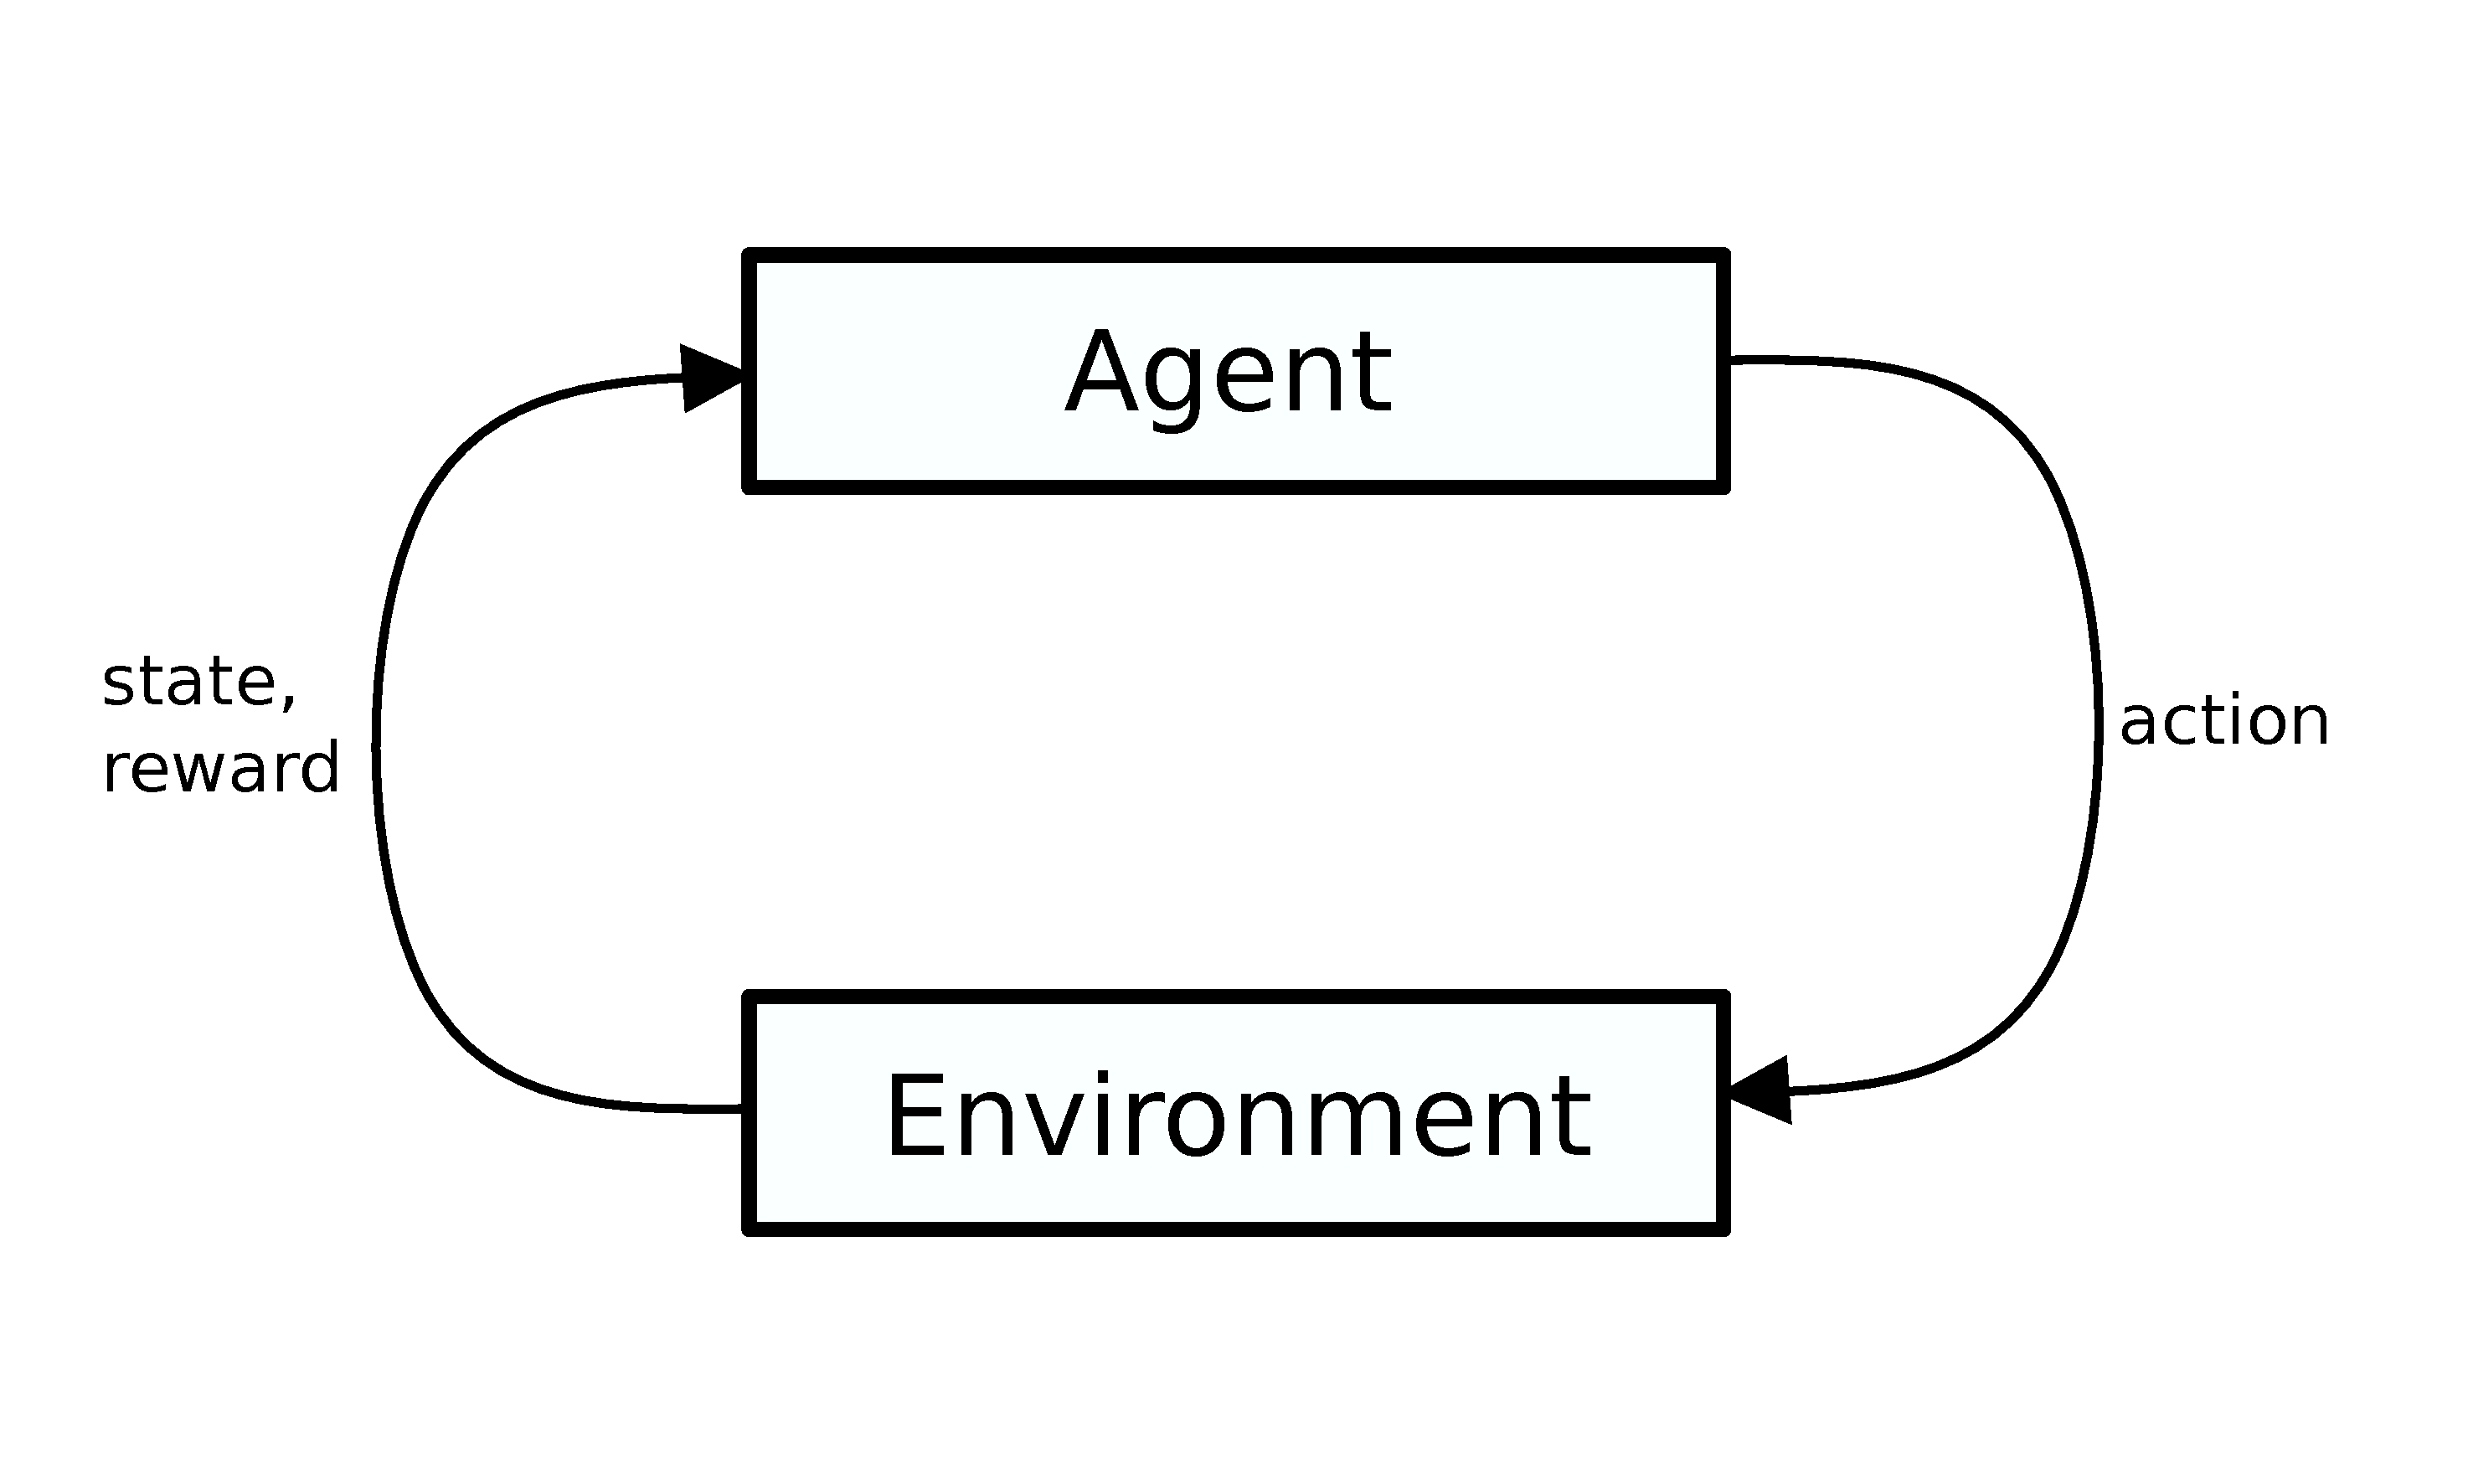
\includegraphics[width=10cm]{submission/figures/figure-basics.pdf}
    \caption{The agent chooses an action and performs it. The environment returns the next state and a reward.} \label{fig-basics}
\end{figure}

The standard framework of reinforcement learning is made up of an environment and an agent following a \textit{Markov decision process} \cite{sutton2018reinforcement}. The environment consists of the state space $\mathcal{S}$ and action space $\mathcal{A}$. Each state-action pair has associated transition probabilities $P(s'|s,a)$ which determines the next state, and each transition has a reward $R(s,a,s')$. The Markov decision process also makes use of the discount factor $\gamma \in [0,1]$. In each state, the agent uses a policy $\pi$ to select its next action, upon which the environment returns the next state (chosen using the probabilistic transition function) and the reward associated with that transition (see Fig. \ref{fig-basics}) \cite{sutton2018reinforcement}.

Different algorithms exist for determining the optimal policy in a given situation. Traditional examples include Q-learning (off-policy) and SARSA (on-policy) \cite{sutton2018reinforcement,watkins1992q}. These algorithms commonly use Bellman equations to assign a Q-value to state-action pairs, which are then used to determine the optimal action in each state \cite{sutton2018reinforcement}.

For example, this Bellman equation defines the Q-value of a state-action pair based on the expected outcome:

$$Q(s,a) = \mathbb{E} R(s,a) + \gamma \mathbb{E} Q(s',a')$$

Exploration is a central concept to reinforcement learning because the agent should know as much information as possible about the environment in order to navigate it. An policy that is too greedily focused on short-term benefits can miss superior solutions if they are not immediately obvious. On the other hand, a policy that focuses only on exploration will struggle to follow an optimal path \cite{sutton2018reinforcement}. The larger the environment, the more time will be taken up by exploration, increasing the need for efficiency in this regard.

\textit{Deep reinforcement learning} combines traditional reinforcement learning with deep learning, using RL methods to train neural networks. Established deep RL algorithms include Deep Q-Networks (DQN) \cite{mnih2013playing} and Deep Deterministic Policy Gradient (DDPG) \cite{lillicrap2015continuous}, which both make use of an experience replay buffer. This replay buffer is used to store transitions that are then used to train the network at a later time. The replay buffer is maintained and not reset between training episodes.

\section{Technologies}

The following five technologies show different new approaches to solving the varied reinforcement learning challenges. Each section contains an explanation of the motivation behind the approach, a summary of the methods of the technology, and a brief overview of some of the evaluations done by the original authors.

\subsection{Distributional Reinforcement Learning}

\subsubsection{Motivation}

Ordinarily, the Bellman equation only considers the expected return of a policy. Two policies with the same expected return are considered equivalent, even if the underlying probability distributions are different and can lead to different results. This, of course, means that information that could be useful for solving a problem is lost.

\textit{Distributional reinforcement learning} (DistRL) \cite{bellemare2017distributional} seeks to rectify this problem by considering the value distribution $Z$.

\subsubsection{Method}

\begin{figure}
    \centering
    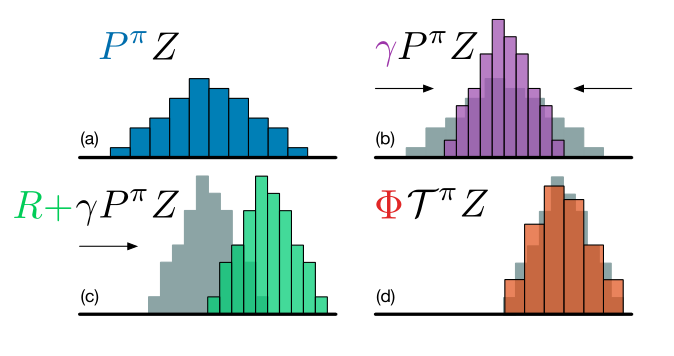
\includegraphics[width=10cm]{submission/figures/figure-distr.png}
    \caption{(a) An example of a value distribution (here, $P^\pi Z(s,a) = Z(s',a')$); (b) The distribution contracts when multiplied with the discount factor; (c) It is shifted by adding the reward; (d) Projection step. \cite{bellemare2017distributional} }
    \label{fig-distr}
\end{figure}

The value distribution can be defined by the distributional Bellman equation (see also Fig. \ref{fig-distr}a-c): $$Z(s,a) \overset{D}{=} R(s,a) + \gamma Z(s',a')$$

$Z(s,a)$ is a probability distribution that is influenced by three sources of randomness: The reward $R$, which is treated as a random variable in this model, the policy's transition probability distribution $P^\pi$, and the next state's value distribution $Z(s',a')$ \cite{bellemare2017distributional}.

While the fact that $Q(s,a) = \mathbb{E} Z(s,a)$ may suggest that a distributional algorithm should lead to the same policy as a traditional method, this is not the case. By incorporating random effects, the value distribution is a richer source of information about the environment than the expected value alone. This can lead to better results than the traditional approach, but unfortunately it cannot be guaranteed that the value distribution converges in all cases, unlike the regular expected value. This, in turn, means that policies based on the distribution may be unstable, which is a significant limitation \cite{bellemare2017distributional}.

In addition, some approximations are necessary to implement distributional RL algorithms in practice due to the complexity of the value distribution. A discrete distribution should be used to allow easier computation, and a projection (see Fig. \ref{fig-distr}d) can be used to fit the distribution onto consistent discrete supports after each step. With these simplifications it is possible to define a \textit{categorical algorithm} which can be used for training a policy \cite{bellemare2017distributional}.

\subsubsection{Evaluation}

When evaluated on the Atari 2600 Arcade Learning Environment (ALE), an implementation of distributional RL based on DQN (\textit{categorical DQN}) was capable of impressive results. Using a finer discrete approximation of the value distributions, with more supports (atoms) and a lower distance between them, produced the most consistently good outcomes. The new algorithm was able to outperform existing algorithms, including regular DQN, in multiple cases — and in particular in the game \textsc{Seaquest}, which was one of the more challenging tasks for DQN \cite{mnih2013playing}, and where the distributional implementation succeeded at beating the previous state of the art \cite{bellemare2017distributional}.

\subsection{Asynchronous Deep Reinforcement Learning}

\subsubsection{Motivation}

While existing deep RL algorithms using experience replay are very powerful, the technique is computationally expensive. \textit{Asynchronous deep RL} (ADRL) promises to require less specialized hardware and achieve better performance than DQN or other deep RL algorithms \cite{mnih2016asynchronous}.

\subsubsection{Method}

This approach can be applied to both on-policy and off-policy algorithms.  Four examples of asynchronous algorithms are: Asynchronous one-step Q-learning, asynchronous n-step Q-learning, asynchronous one-step SARSA, and asynchronous advantage actor-critic (A3C) \cite{mnih2016asynchronous}.

ADRL runs on a CPU with multiple threads. There are shared parameters $\theta$ and a global counter $T$. Each thread runs a separate actor-learner agent with its own initial state and exploration policy, and each has a thread-specific counter $t$ as well as well as thread-specific parameters depending on the specific algorithm. These include a set of gradients $d\theta$, which are used to periodically make asynchronous updates to the global $\theta$, and a local copy of the shared parameters, which is also updated periodically. Because these updates are done asynchronously, each agent's copy of the environment may differ slightly at any given time. However thanks to the different initial states and exploration policies, they will usually be exploring different parts of the environment with little overlap, which has a stabilizing effect \cite{mnih2016asynchronous}.

While the above properties are shared by all four asynchronous algorithms, the details of how the values and gradients are calculated differs based on the original algorithms that they are derived from (i.e. Q-learning, SARSA, etc.).

\subsubsection{Evaluation}

This architecture has a number of benefits \cite{mnih2016asynchronous}:

\begin{itemize}
    \item The parallel execution of multiple agents leads to reduced training time that scales nearly linearly with the number of threads.
    \item By running on a single CPU with asynchronous updates, communication costs for updating the parameters are minimized compared to some other parallel methods, e.g. \textit{Gorila}.
    \item Compared to DQN or other experience replay-based methods, the asynchronous approach is not limited to off-policy algorithms.
\end{itemize}

Experiments conducted in the Atari 2600 ALE show how quickly the asynchronous algorithms can learn, as they were often able to match or outperform DQN with less time required for training. This effect was especially pronounced in the game \textsc{Breakout}. Out of the four algorithms, A3C in particular can run on a single 16-core CPU and achieve comparable or superior results to DQN trained on GPUs while spending half the time on training. The algorithm also outmatched the score for \textit{Gorila}, which was trained on 100 machines. Other tests using different environments confirmed that A3C is the most powerful of the four asynchronous algorithms \cite{mnih2016asynchronous}.

\subsection{Hindsight Experience Replay}

\subsubsection{Motivation}

Ordinarily, solving complex problems with reinforcement learning requires a complicated reward function.  The challenges of producing such an optimized reward function could be avoided by using sparse and binary rewards, e.g. $-1$ for not reaching a goal and $0$ for reaching it.

\textit{Hindsight Experience Replay} (HER) \cite{andrychowicz2017hindsight} is an approach that allows learning from such sparse and binary rewards in a multi-goal setting. The technique is used on top of existing off-policy deep RL algorithms such as DQN or DDPG. As the name suggests, it makes use of and improves upon the experience replay mechanism of these algorithms.

\subsubsection{Method}

In addition to using an on-policy algorithm, another prerequisite of HER is the use of \textit{Universal Value Function Approximators} (UVFA) \cite{schaul2015universal}, which allow multi-goal learning. UVFA is used to define different reward functions for any possible goals, i.e. $R(s,a,g)$, which is simple if all the rewards are sparse and binary. This leads to a Q-value function that also depends not only on on the state and action, but on the agent's goal as well: $Q(s,a,g)$ \cite{andrychowicz2017hindsight}

In each training episode, the HER algorithm samples an initial state $s_0$ and a goal $g$ which it attempts to reach using the policy derived from a chosen learning algorithm (e.g. DDPG), taking a set number of successive actions. Then, all its transitions (meaning beginning state $s_t$, action $a_t$, goal $g$, reward $r_t$, next state $s_{t+1}$; with $r_t$ = $R(s_t,a_t,g)$) are stored in the experience replay buffer, as is standard. Additionally, out of all the states that the agent passed through during the episode, a subset is chosen as additional goals. For each additional goal $g'$, HER creates another copy of each transition where $g'$ is saved instead of $g$ and $r' = R(s_t,a_t,g')$ is saved instead of $r_t$. These additional, modified transitions were not made during the episode, but they represent rewards that could have been achieved by the agent's actions if the goal had been different. They are also stored in the replay buffer \cite{andrychowicz2017hindsight}.

This results in many more transitions being added to the replay buffer, which is additional information about the environment for the agent to learn from. Whereas a traditional agent would have learned very little from sparse rewards, the evaluation of transitions with respect to multiple goals (some of which were actually achieved) during one single episode allows the HER agent to improve its policy even when the original goal isn't reached \cite{andrychowicz2017hindsight}.

\subsubsection{Evaluation}

Experiments in a robotics environment with sparse binary rewards show that DDPG + HER is very capable at solving a number tasks that are entirely beyond the capabilities of DDPG alone. This is especially true in a multi-goal case, but even with only a single goal it was able to outperform simple DDPG. When evaluated using shaped rewards, however, HER failed almost completely (as did DDPG in this environment) \cite{andrychowicz2017hindsight}.

\subsection{Feudal Networks}

\subsubsection{Motivation}

\textit{FeUdal Networks} (FuNs) combine previously existing feudal RL methods \cite{dayan1993feudal} with modern deep RL. It is a hierarchical model composed of two levels, the Manager and the Worker, which are modeled as separate modules \cite{vezhnevets2017feudal}.

\subsubsection{Method}

In essence, the Manager's role is to provide goals for the Worker to train with, while the Worker takes primitive actions based on these goals. The Manager therefore works at a reduced temporal resolution, as each goal produced by the Manager corresponds to many actions taken by the Worker. Beyond the goal being communicated to the Worker by the Manager, the two modules do not exchange any gradients or other data and train their policies independently \cite{vezhnevets2017feudal}. With time, the Manager thus learns to generate better goals that guide the Worker more successfully.

The practical implementation of the model is based on the long short-term memory (LTSM) type of recurrent neural network \cite{hochreiter1997long,vezhnevets2017feudal}. The worker uses a regular LTSM, while the manager's architecture is a variation termed \textit{dilated LTSM}. Both share a common perceptual module which provides observations $z$ from the environment. The manager uses these observations and a new transition policy gradient, which is a modification of the policy gradient training method and takes advantage of the expectation that the Worker will eventually follow the Manager's directions, to train its policy. The manager produces directional goals, meaning that the Worker is rewarded for moving in the correct direction, rather than only for reaching a goal state. In order to achieve temporal abstraction and smoother directional goals, several goals are combined using a linear transformation. This combined goal, together with the environmental observation and the Worker policy, is used to generate the next action. The Worker trains its policy individually using the policy gradient method \cite{vezhnevets2017feudal}. 

\subsubsection{Evaluation}

Experimental evaluation of FuNs using the Arcade Learning Environment shows that the new model is able to outperform conventional LTSM in many games, notably including \textsc{Montezuma's Revenge}, \textsc{Enduro}, and \textsc{Frostbite}. However, it produced inferior results at \textsc{Breakout} and \textsc{Seaquest}, showing that the added complexity of the hierarchical model isn't always required and can, in fact, hamper learning in some cases \cite{vezhnevets2017feudal}.

\subsection{Hierarchical Actor-Critic}

\begin{figure}
    \centering
    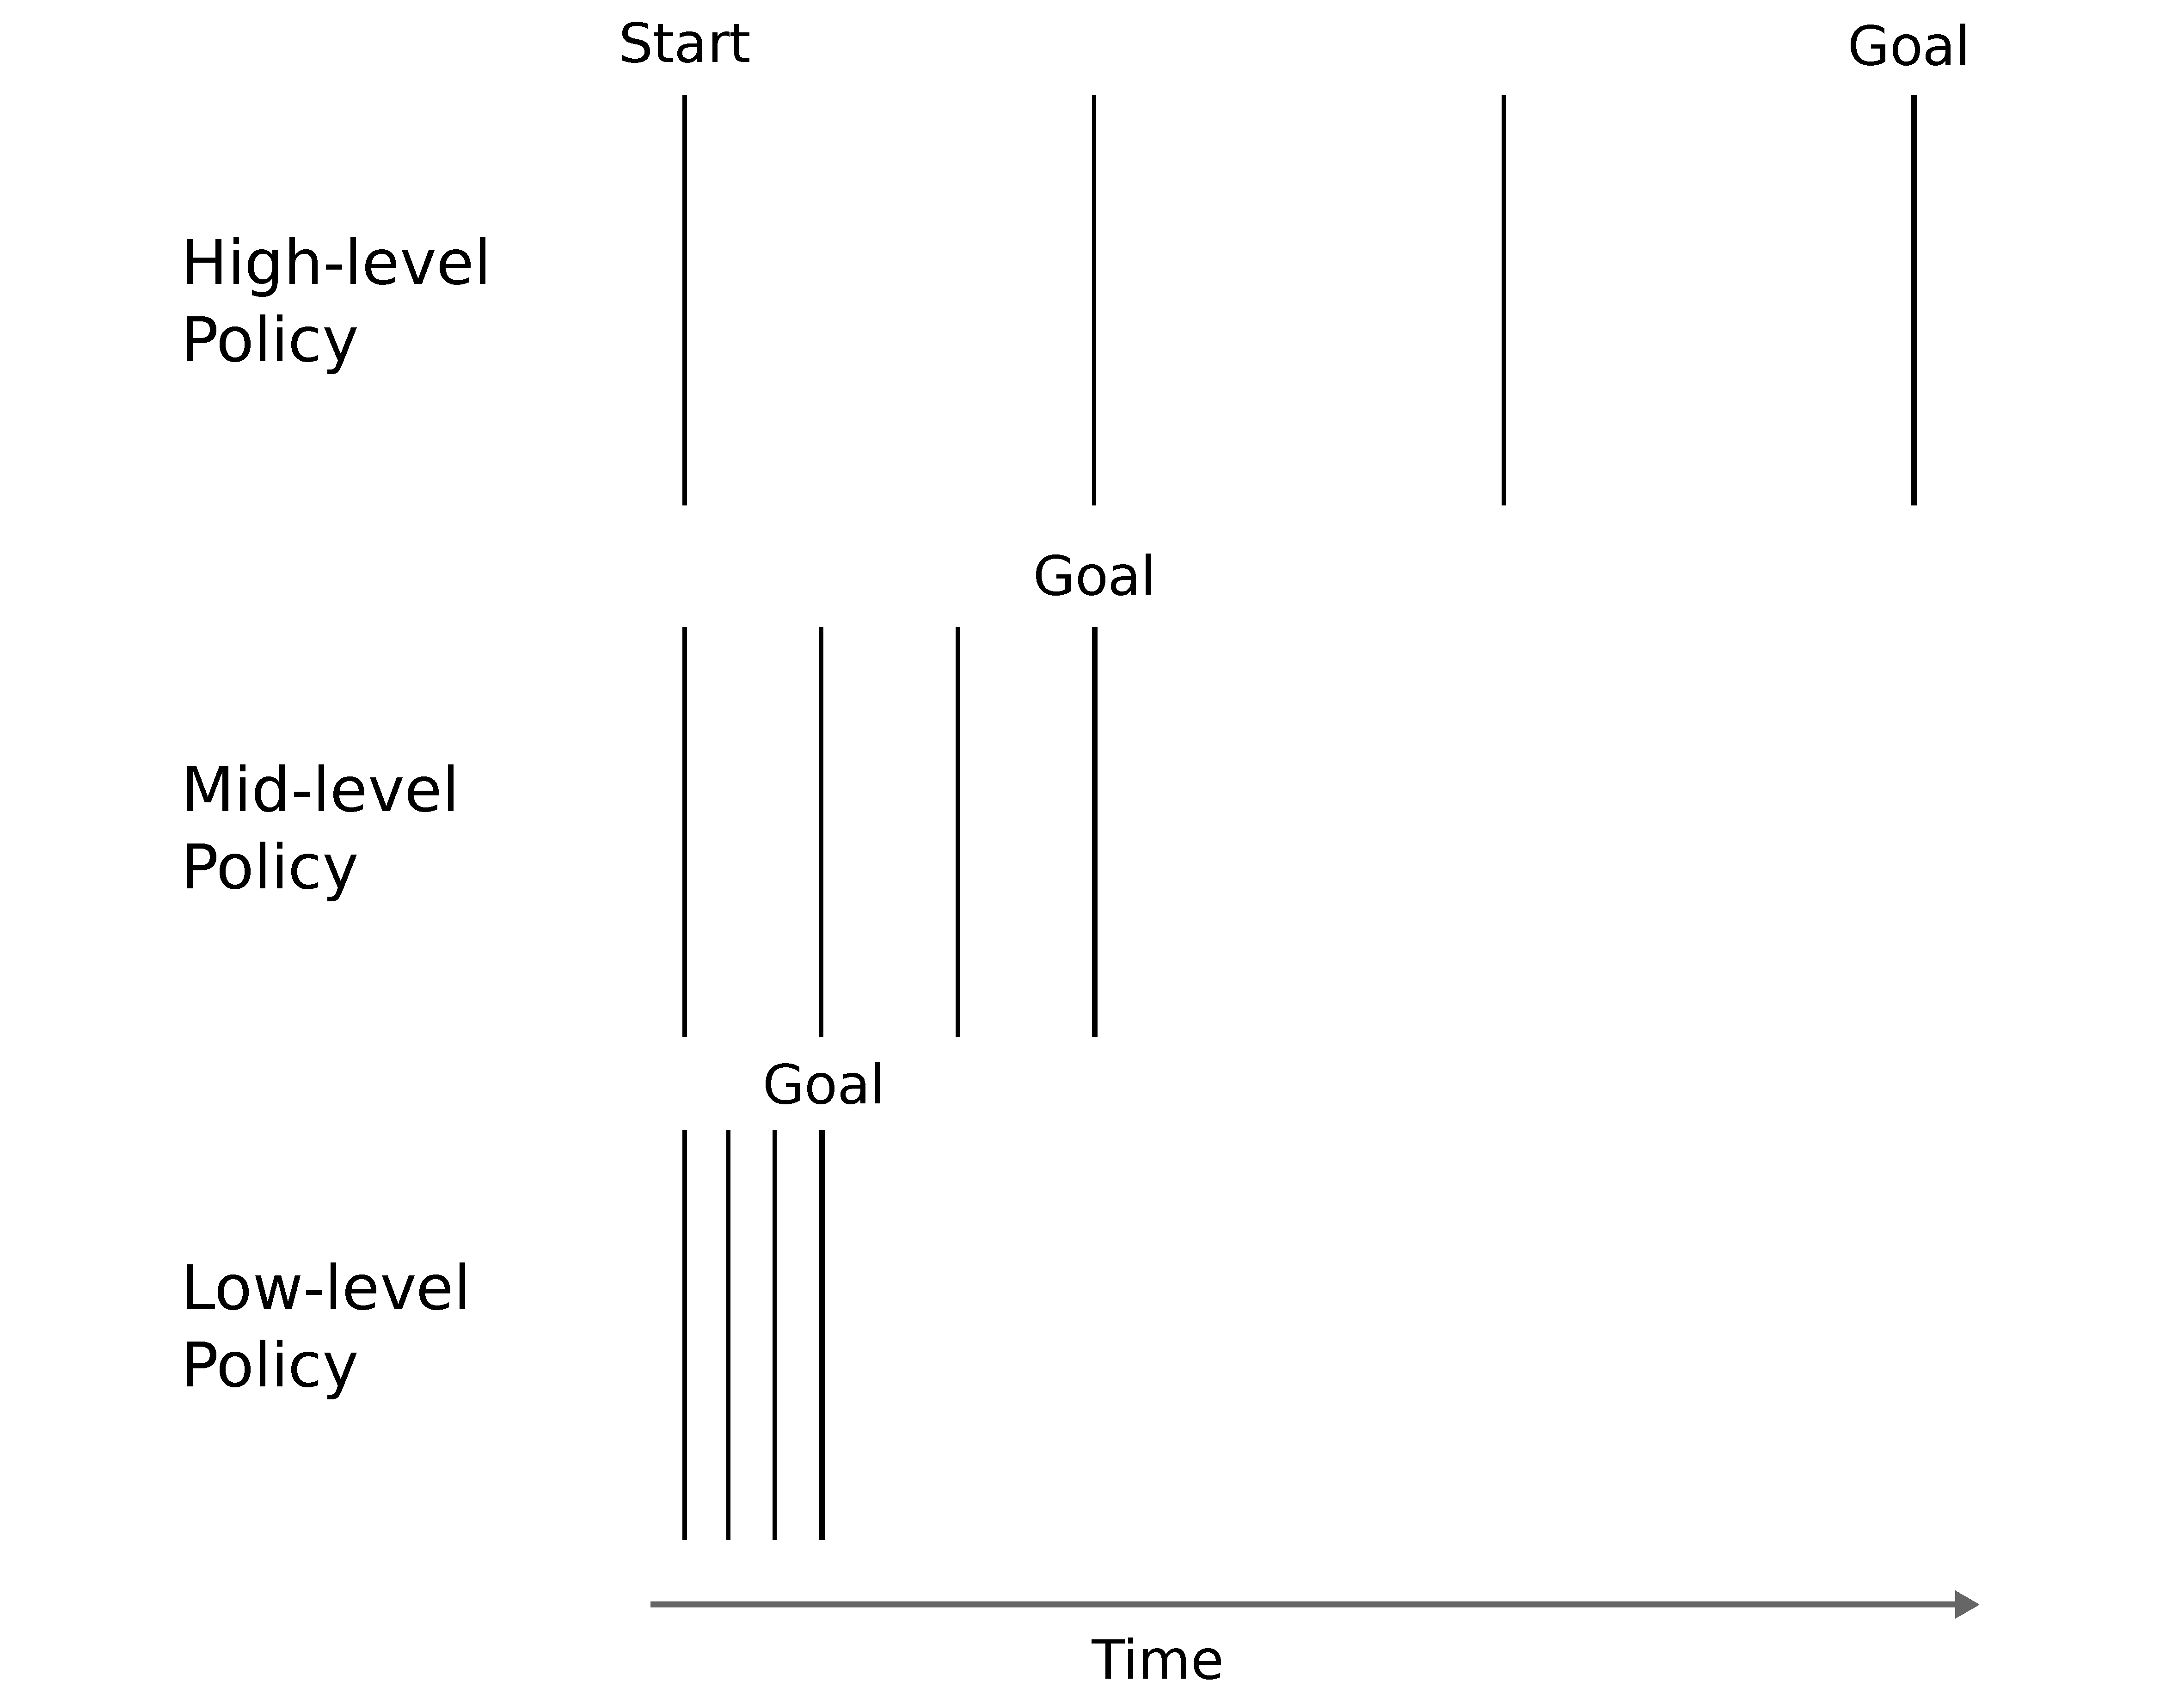
\includegraphics[width=10cm]{submission/figures/figure-hactask.pdf}
    \caption{An example of HAC with three layers dividing a task. Each step at a higher level corresponds to multiple steps for the lower level. \cite{levy2017hierarchical}}
    \label{fig-hactask}
\end{figure}

\begin{figure}
    \centering
    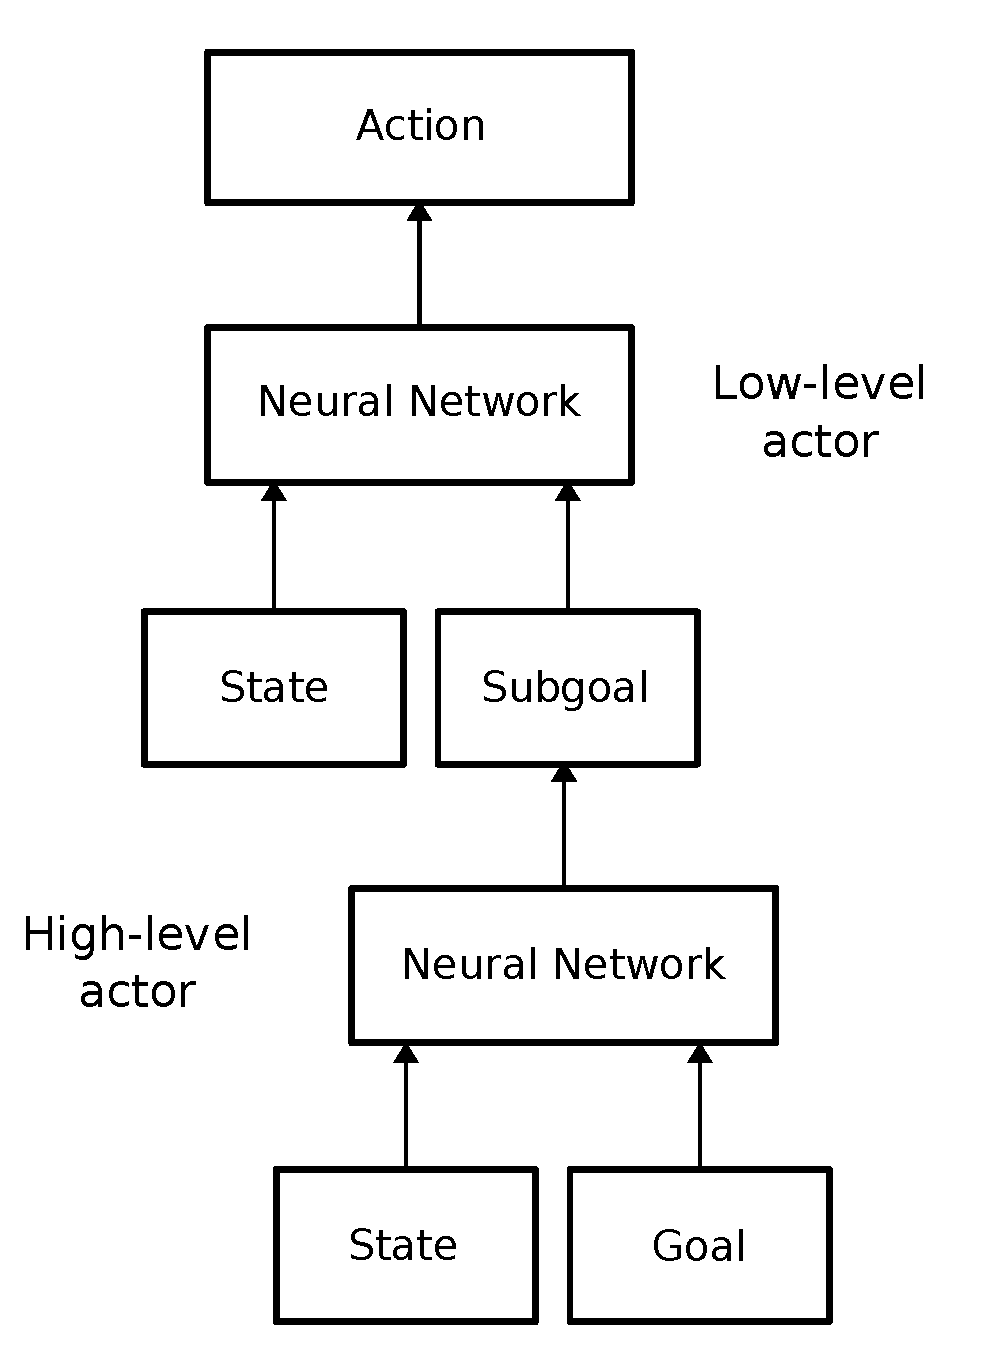
\includegraphics[width=6cm]{submission/figures/figure-hierarchy.pdf}
    \caption{An example of the HAC structure with two layers. The high-level actor uses its state and the overall goal to generate subgoals, which the low-level actor uses together with its own state to generate actions. \cite{levy2017hierarchical}}
    \label{fig-hierarchy}
\end{figure}

\subsubsection{Motivation}

While the benefits of hierarchical reinforcement learning are often significant, most previous hierarchical approaches, including FuNs, can only operate on discrete action spaces. They are unable to effectively learn at higher levels of abstraction if the action space is continuous. Furthermore, for a hierarchical algorithm to be as efficient as possible, the work should be divided evenly between the different agents. Many previous methods unfortunately struggle to do so. \textit{Hierarchical Actor-Critic} (HAC) is a new technique for hierarchical RL specifically aimed at improving these two aspects \cite{levy2017hierarchical}.

\subsubsection{Method}

Like FuNs, HAC divides tasks on a temporal scale between its multiple layers. Unlike FuNs, which operate with two levels, HAC is designed for a variable number of layers: There is always a bottom layer, which takes atomic actions from the action space $\mathcal{A}$. On top of this there can be any number of subgoal layers. The subgoal layers select subgoals as their actions, which then become the next goal for the next lower layer to reach (see Fig. \ref{fig-hactask}, \ref{fig-hierarchy}) \cite{levy2017hierarchical}.

The practical implementation of this architecture uses DDPG, which is an actor-critic algorithm (hence the name), and Hindsight Experience Replay to train the policy of each layer. HER is incorporated to take advantage of its ability to efficiently learn with multiple goals using sparse rewards \cite{levy2017hierarchical}.

The algorithm uses a structure of several nested loops, each representing a layer. The outermost loop (top layer, or layer $n$) receives an initial state and the actual goal of the task. It uses these parameters and its policy to choose a subgoal. This subgoal is passed to the next loop (layer $n-1$), where it becomes the new goal, which is used along with that layer's own policy and state to sample new subgoals for the next lower layer, and so on. The innermost loop (bottom layer, or layer $0$) uses its policy to generate atomic actions rather than subgoals. Once the bottom layer has reached a goal, or has taken a predetermined number of steps without success, the loop terminates. The next higher layer (layer $1$) then generates a new subgoal for the lower layer, and keeps doing so until it reaches its goal or until it also exhausts its preset number of steps. The nested algorithm continues in this fashion until the top layer has reached the overall goal or exhausted all its steps, at which point the training episode is concluded, the actor-critic networks are updated, and a new initial state and goal can be sampled for the next episode \cite{levy2017hierarchical}.

By limiting each layer to taking a certain number of steps at a time, which in most cases will not be enough for the lower layers to reach the overall goal on their own, the system is prevented from letting the bottom layer do all the work. At the same time, the higher layers are penalized for generating unreachable goals. Combined, these incentives encourage the system to divide its tasks equitably. The aforementioned step-count restriction also means that each layer only has to learn a relatively short policy, which will be more effective than a single agent learning one long policy \cite{levy2017hierarchical}.

\subsubsection{Evaluation}

Versions of the HAC algorithm with one and two subgoal layers were tested and compared to a baseline HER + DDPG ("0 subgoal layers") algorithm using tasks in a Mujoco physics simulation. The results show that the HAC algorithms outperformed the baseline in every case. The agent with 2 subgoal layers was superior to the 1 subgoal layer agent in most experiments, but the version with a single subgoal layer was able to reach better results in one trial  \cite{levy2017hierarchical}. It can be concluded that hierarchical learning with HAC performs better than the baseline, but adding additional layers is not always worth it. Further experiments with three or more subgoal layers would be needed to check whether this conclusion holds true.

\section{Conclusion}

This review shows the wide variety of approaches that can be used when developing new reinforcement learning algorithms. It is clear that different technologies are created for different situations — a method crafted for one problem might not be suitable for another.

The literature on distributional RL shows the value of looking beyond the traditional Bellman equations and using the entire value distribution to train agents. That said, there is still work to be done as more efficient ways to work with value distributions should be investigated. It is likely possible for distributions to be introduced to more complex learning algorithms which might require fewer approximations and workarounds.

One of the significant contributions of asynchronous deep RL is that it shows how effective policies can be trained much more efficiently and without requiring as much specialized hardware. Such improvements are valuable for solving increasingly complex problems with reinforcement learning and may in the future allow deep RL to be deployed on a larger number of devices, including mobile devices.

Another benefit of ADRL is that different reinforcement learning algorithms can potentially be adapted to fit the asynchronous framework. Further research may investigate how the technology can be applied to other RL algorithms and how this would impact learning performance.

Hindsight Experience Replay appears to be especially promising due to the way it is used on top of different existing deep RL algorithms and the fact that it allows learning in situations that would be completely out of reach otherwise. The simplicity of sparse rewards opens the door to solving tasks which previously required complicated reward engineering, which appears to be especially useful for robotics applications. HAC also shows that HER is flexible, it can be combined with a variety of other technologies and form the foundation of more specialized solutions. More such developments can be the target of additional research.

Both of the hierarchical methods have similar goals, namely to divide the task between their layers on a temporal scale and to allow each layer to learn its own policy as effectively as possible. And while they both approach these goals using deep RL technology, their specific implementations are quite different: Feudal Networks implements a clear distinction between Manager and Worker, both using entirely different methods to train and apply their policies. Hierarchical Actor-Critic on the other hand has every layer use the same fundamental architecture, which has the benefit of flexibility as more layers can be added as needed.

Further research may show how FuNs might be expanded to increase the level of abstraction. When it comes to HAC, the performance of a model with more than two subgoal layers should be examined (though it would likely lead to diminishing returns), and the technology's effectiveness could be compared with other hierarchical and non-hierarchical approaches. Even a comparison between FuNs and HAC may be interesting and highlight their strengths and weaknesses in different use cases.

One final potential avenue of future research may be a combination of two of the technologies examined here. Even though ADRL is specifically designed without experience replay, it has already been suggested that experience replay could be incorporated into the asynchronous framework \cite{mnih2016asynchronous}. This would open the doors to a possible implementation of asynchronous Hindsight Experience Replay which, if successful, may combine the benefits of both technologies: A much more resource-efficient way to learn sparse reward tasks.

%
% ---- Bibliography ----
%
% BibTeX users should specify bibliography style 'splncs04'.
% References will then be sorted and formatted in the correct style.

\bibliographystyle{splncs04}
\bibliography{bibliography}

\end{document}